\chapter{Results and Discussion}\label{chap:results}
All numbers below come from logged runs on the hardware in Chapter~3. Unless stated otherwise, the seed is 42.

\section{Classifier accuracy}
The project requirement was at least 95\% accuracy and at least 0.95 macro F1. The earlier classifier comparison, on a 500{,}000-row class-balanced sample of the base features, gave 0.891 accuracy and 0.887 macro F1. On all 1.9 million rows with the natural class distribution, the same base features give 0.964 accuracy but still only 0.887 macro F1, because the application-layer attacks are confused with each other.

The final classifier is trained on 1{,}429{,}825 packets and tested on 397{,}073 packets from connections it never saw (Table~\ref{tab:datascale}).

\subsection{Ambiguity ceiling}
Before tuning the model, we measured how many rows are impossible to separate with each feature set (Table~\ref{tab:ceiling}). With the 91 base features, 2.31\% of rows share an identical feature vector with a row of a different class, which caps macro recall at 0.969 for \emph{any} per-packet classifier. The new features bring the ambiguous share down to 0.01\%.
\begin{table}[H]
\centering
\renewcommand{\arraystretch}{1.2}
\begin{tabular}{|l|c|c|c|c|}
\hline
\textbf{Feature set} & \textbf{Features} & \textbf{Ambiguous} & \textbf{Ceiling acc.} & \textbf{Ceiling macro rec.} \\ \hline
Base & 91 & 2.31\% & 0.9875 & 0.9692 \\ \hline
+ service port & 92 & 0.29\% & 0.9985 & 0.9940 \\ \hline
+ content + flow & 130 & 0.01\% & 0.9999 & 0.9997 \\ \hline
\end{tabular}
\caption{Ambiguity ceiling per feature set (all rows, after de-duplication)}
\label{tab:ceiling}
\end{table}

\subsection{Effect of each feature group}
Table~\ref{tab:progression} and Figure~\ref{fig:progression} add the feature groups one at a time, on the strict flow-grouped split. The service port mainly fixes Normal versus attack traffic. The content features add little on their own, because only a small share of packets carries content. The flow features give the largest jump, because they pass a connection's content and behaviour on to its content-free packets. Class weighting then stabilises the rare Fingerprinting class.
\begin{table}[H]
\centering
\renewcommand{\arraystretch}{1.2}
\begin{tabular}{|l|c|c|c|c|}
\hline
 & \multicolumn{2}{c|}{\textbf{Random split}} & \multicolumn{2}{c|}{\textbf{Flow-grouped split}} \\ \hline
\textbf{Features} & \textbf{Accuracy} & \textbf{Macro F1} & \textbf{Accuracy} & \textbf{Macro F1} \\ \hline
Base (91) & 0.9638 & 0.8868 & 0.9637 & 0.8892 \\ \hline
+ service port (92) & 0.9802 & 0.9245 & 0.9803 & 0.9236 \\ \hline
+ content (110) & 0.9802 & 0.9268 & 0.9802 & 0.9232 \\ \hline
+ flow (130) & 0.9977 & 0.9879 & 0.9975 & 0.9808 \\ \hline
\textbf{+ class weights (final)} & \textbf{0.9976} & \textbf{0.9867} & \textbf{0.9972} & \textbf{0.9828} \\ \hline
\end{tabular}
\caption{Accuracy and macro F1 as feature groups are added (LightGBM, all rows, 80/20)}
\label{tab:progression}
\end{table}
\begin{figure}[H]
\centering
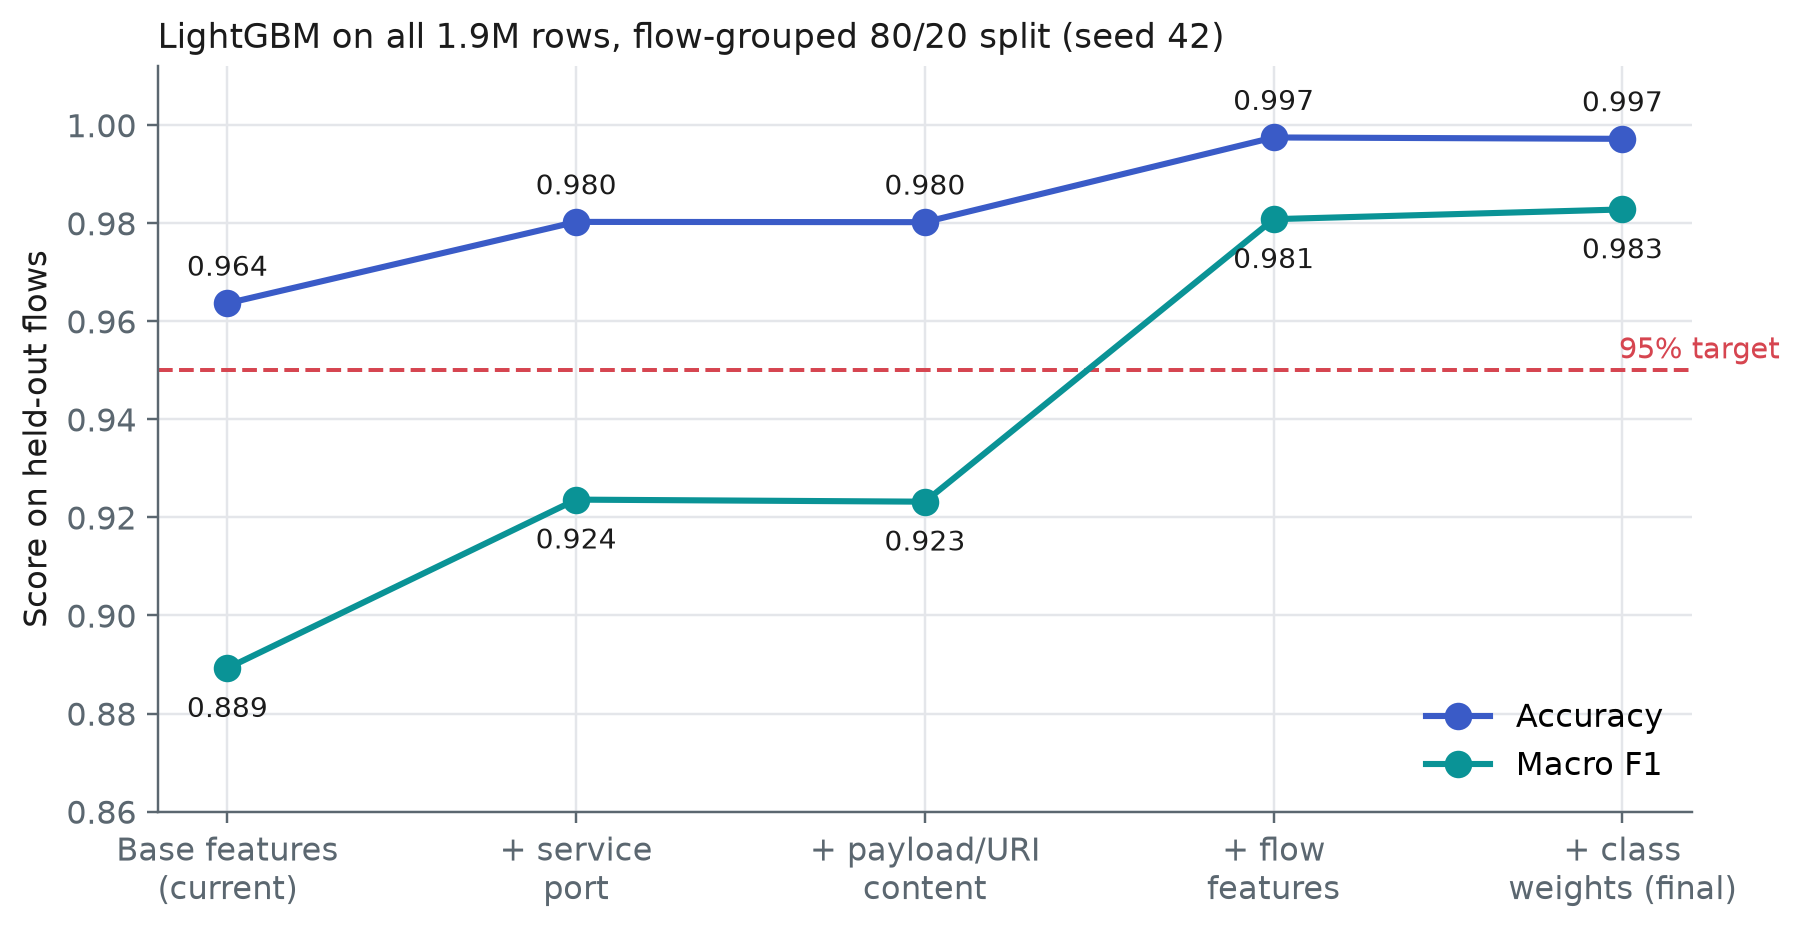
\includegraphics[width=0.92\linewidth]{figures/accuracy_progression.png}
\caption{Accuracy and macro F1 on held-out flows as each feature group is added}
\label{fig:progression}
\end{figure}

\subsection{Robustness across seeds, splits and training size}
Table~\ref{tab:seeds} repeats the final configuration with three seeds on both splits. Accuracy stays between 0.9970 and 0.9977, and macro F1 between 0.9828 and 0.9868. Without class weights, the flow-grouped macro F1 was less stable (0.9808, 0.9560, 0.9521), because the Fingerprinting score depended on which of its 156 flows landed in test. Weighting removes that sensitivity.

\begin{table}[H]
\centering
\renewcommand{\arraystretch}{1.2}
\begin{tabular}{|l|c|c|c|}
\hline
\textbf{Split / seed} & \textbf{42} & \textbf{43} & \textbf{44} \\ \hline
Random: accuracy & 0.9976 & 0.9977 & 0.9976 \\ \hline
Random: macro F1 & 0.9867 & 0.9868 & 0.9866 \\ \hline
Flow-grouped: accuracy & 0.9972 & 0.9971 & 0.9970 \\ \hline
Flow-grouped: macro F1 & 0.9828 & 0.9835 & 0.9851 \\ \hline
\end{tabular}
\caption{Final classifier across seeds}
\label{tab:seeds}
\end{table}

Two further checks were run. \textbf{(a) Same sampling as before:} on a 500{,}000-row capped sample drawn the same way as in the earlier boosting-versus-DL comparison, and with the same training settings for both feature sets, accuracy rises from 0.8902 to 0.9919 and macro F1 from 0.8827 to 0.9900. \textbf{(b) Calibration-set size:} in FL-IDS the server trains LightGBM on only a 5\% calibration set. Trained on 5\% of the rows and tested on held-out flows, the new features give 0.9968 accuracy and 0.9791 macro F1, against 0.9624 and 0.8807 for the base features. The gain therefore carries over to the classifier as the federated system actually trains it.

\subsection{Per-class results}
Figure~\ref{fig:perclass} compares per-class F1 before and after. The biggest gains are on exactly the classes that were weak: Uploading (0.76 to 1.00), DDoS\_HTTP (0.76 to 0.97), SQL\_injection (0.80 to 1.00), Password (0.84 to 0.97), XSS (0.85 to 0.98) and Fingerprinting (0.68 to 0.93). Figure~\ref{fig:cm} shows the remaining confusion: Password and DDoS\_HTTP traffic (both HTTP requests to the same server) and Ransomware versus Backdoor (both on port 4321). MITM is a single ARP flow, so it cannot be scored on the flow-grouped split; on the random split its F1 is 0.994.
\begin{figure}[H]
\centering
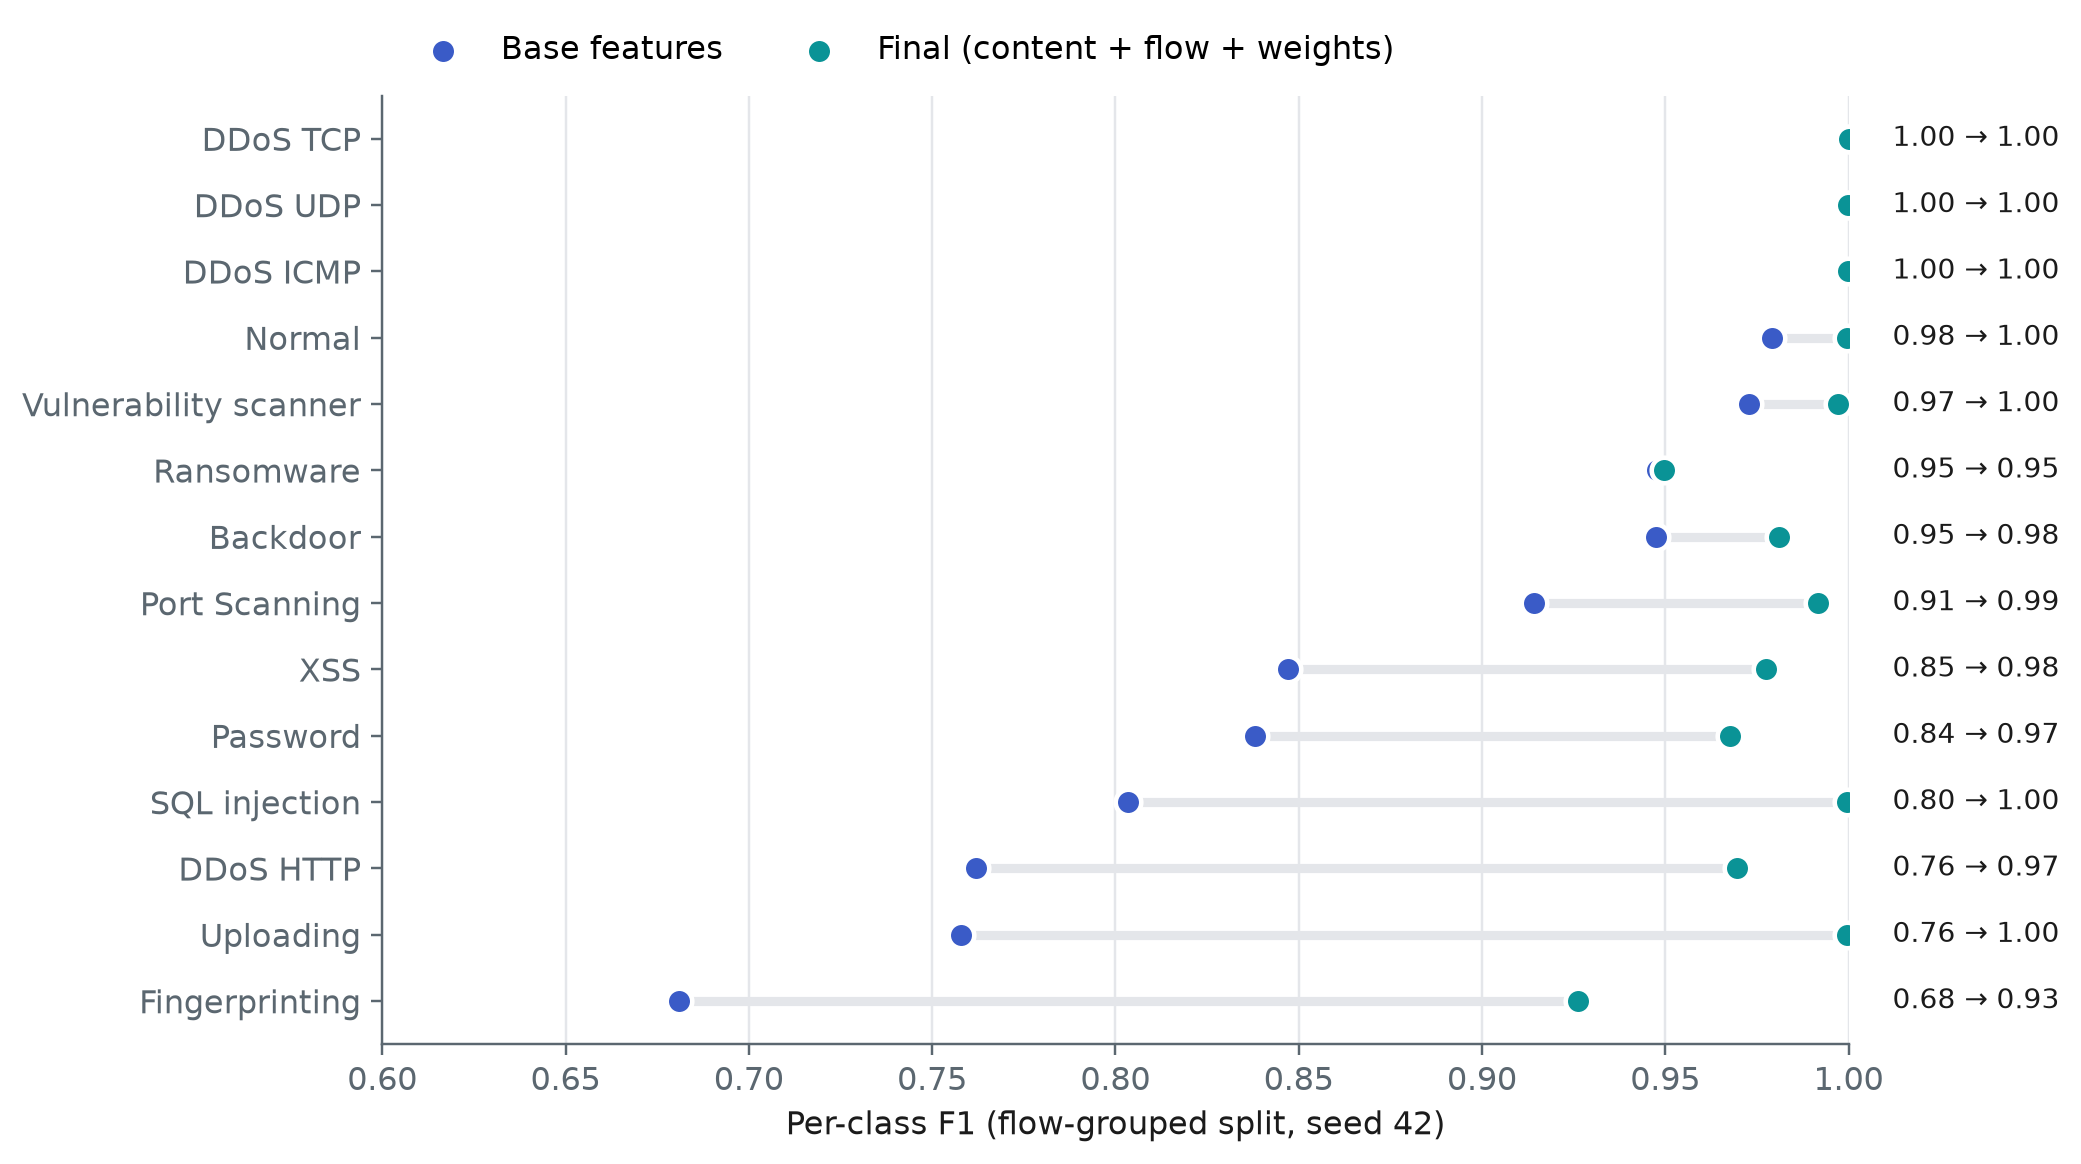
\includegraphics[width=0.88\linewidth]{figures/per_class_f1.png}
\caption{Per-class F1, base features vs.\ final classifier (flow-grouped split)}
\label{fig:perclass}
\end{figure}
\begin{figure}[H]
\centering
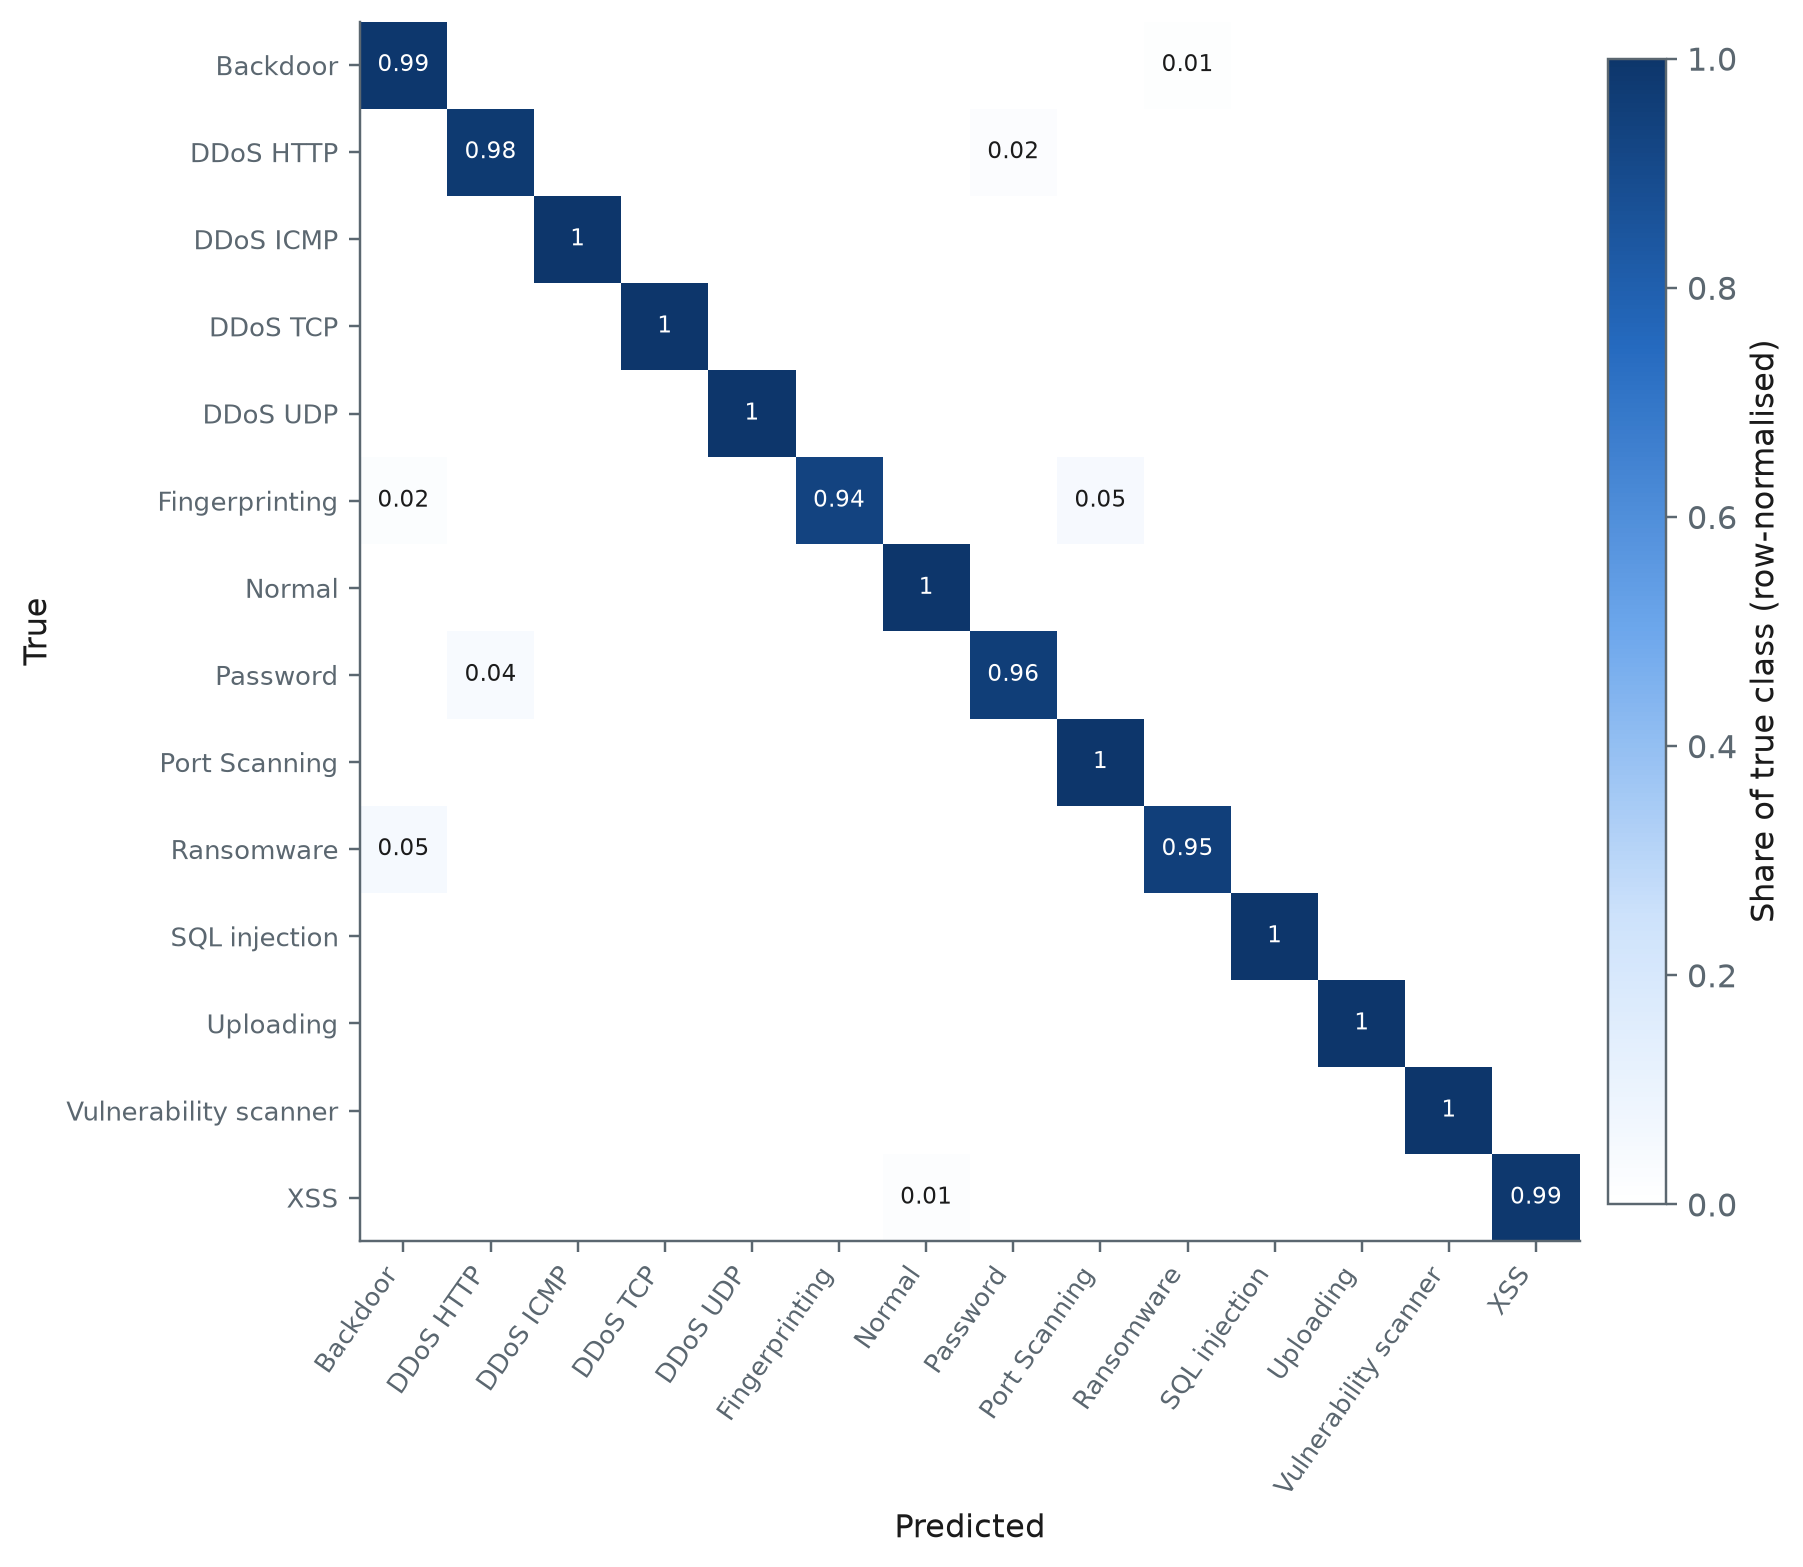
\includegraphics[width=0.8\linewidth]{figures/confusion_final.png}
\caption{Row-normalised confusion matrix of the final classifier (flow-grouped split)}
\label{fig:cm}
\end{figure}

\subsection{Discussion and caveats}
\begin{itemize}
  \item \textbf{Why a flow-grouped split matters.} A random split of packets puts packets of the same connection in both training and test sets. Reporting the stricter split shows that the improvement does not come from memorising connections.
  \item \textbf{The service port is partly a testbed effect.} In Edge-IIoTset, benign traffic is MQTT (port 1883) and VNC (5900) and never HTTP. In a real network with benign web traffic, the port alone would separate much less.
  \item \textbf{Flow features are computed over the whole flow record} (up to 120\,s), the same way as CICFlowMeter. The classifier therefore labels flow records rather than making a decision on the first packet.
  \item The same features are used by the whole federated pipeline and by Phase B. The following sections report the system-level results with them, next to the original 91-feature results.
\end{itemize}

\section{Ablation of the federated pipeline}
Figure~\ref{fig:ablation} and Table~\ref{tab:ablation} compare five variants with 30\% sign-flip attackers (clients 0, 6 and 9), 20 rounds, with the 130-feature pipeline; the original 91-feature results are given in brackets. Known-attack detection is now close to perfect for every variant that includes the classifier (0.996--1.000 macro-recall), so the backstop's value is on \emph{zero-day} attacks: 0.930 macro-recall for the full pipeline against 0.795 for boosting alone. Without the trust filter (plain FedAvg, trimmed mean only) the autoencoder is poisoned again: its stand-alone recall drops to about 0, its validation loss diverges, and zero-day recall falls back to boosting's level (0.795 and 0.799).
\begin{table}[H]
\centering
\footnotesize\setlength{\tabcolsep}{3pt}
\begin{tabular}{|l|c|c|c|c|c|}
\hline
\textbf{Variant} & \textbf{Attack MR} & \textbf{Benign FPR} & \textbf{Detection F1} & \textbf{Zero-day MR} & \textbf{AE-alone MR} \\ \hline
Full pipeline & 1.000 [0.887] & 0.031 & 0.961 & 0.930 [0.731] & 0.712 [0.421] \\ \hline
Plain FedAvg & 0.998 [0.879] & 0.035 & 0.955 & 0.795 [0.595] & 0.002 [0.000] \\ \hline
Trimmed mean only & 0.997 [0.878] & 0.033 & 0.957 & 0.799 [0.539] & 0.000 [0.000] \\ \hline
Autoencoder only & 0.372 [0.191] & 0.030 & 0.465 & 0.577 [0.325] & 0.372 [0.191] \\ \hline
Boosting only & 0.996 [0.875] & 0.000 & 0.998 & 0.795 [0.518] & n/a \\ \hline
\end{tabular}
\caption{Ablation at 30\% malicious clients, 130 features [91 features] (MR = macro-recall)}
\label{tab:ablation}
\end{table}
\begin{figure}[H]
\centering
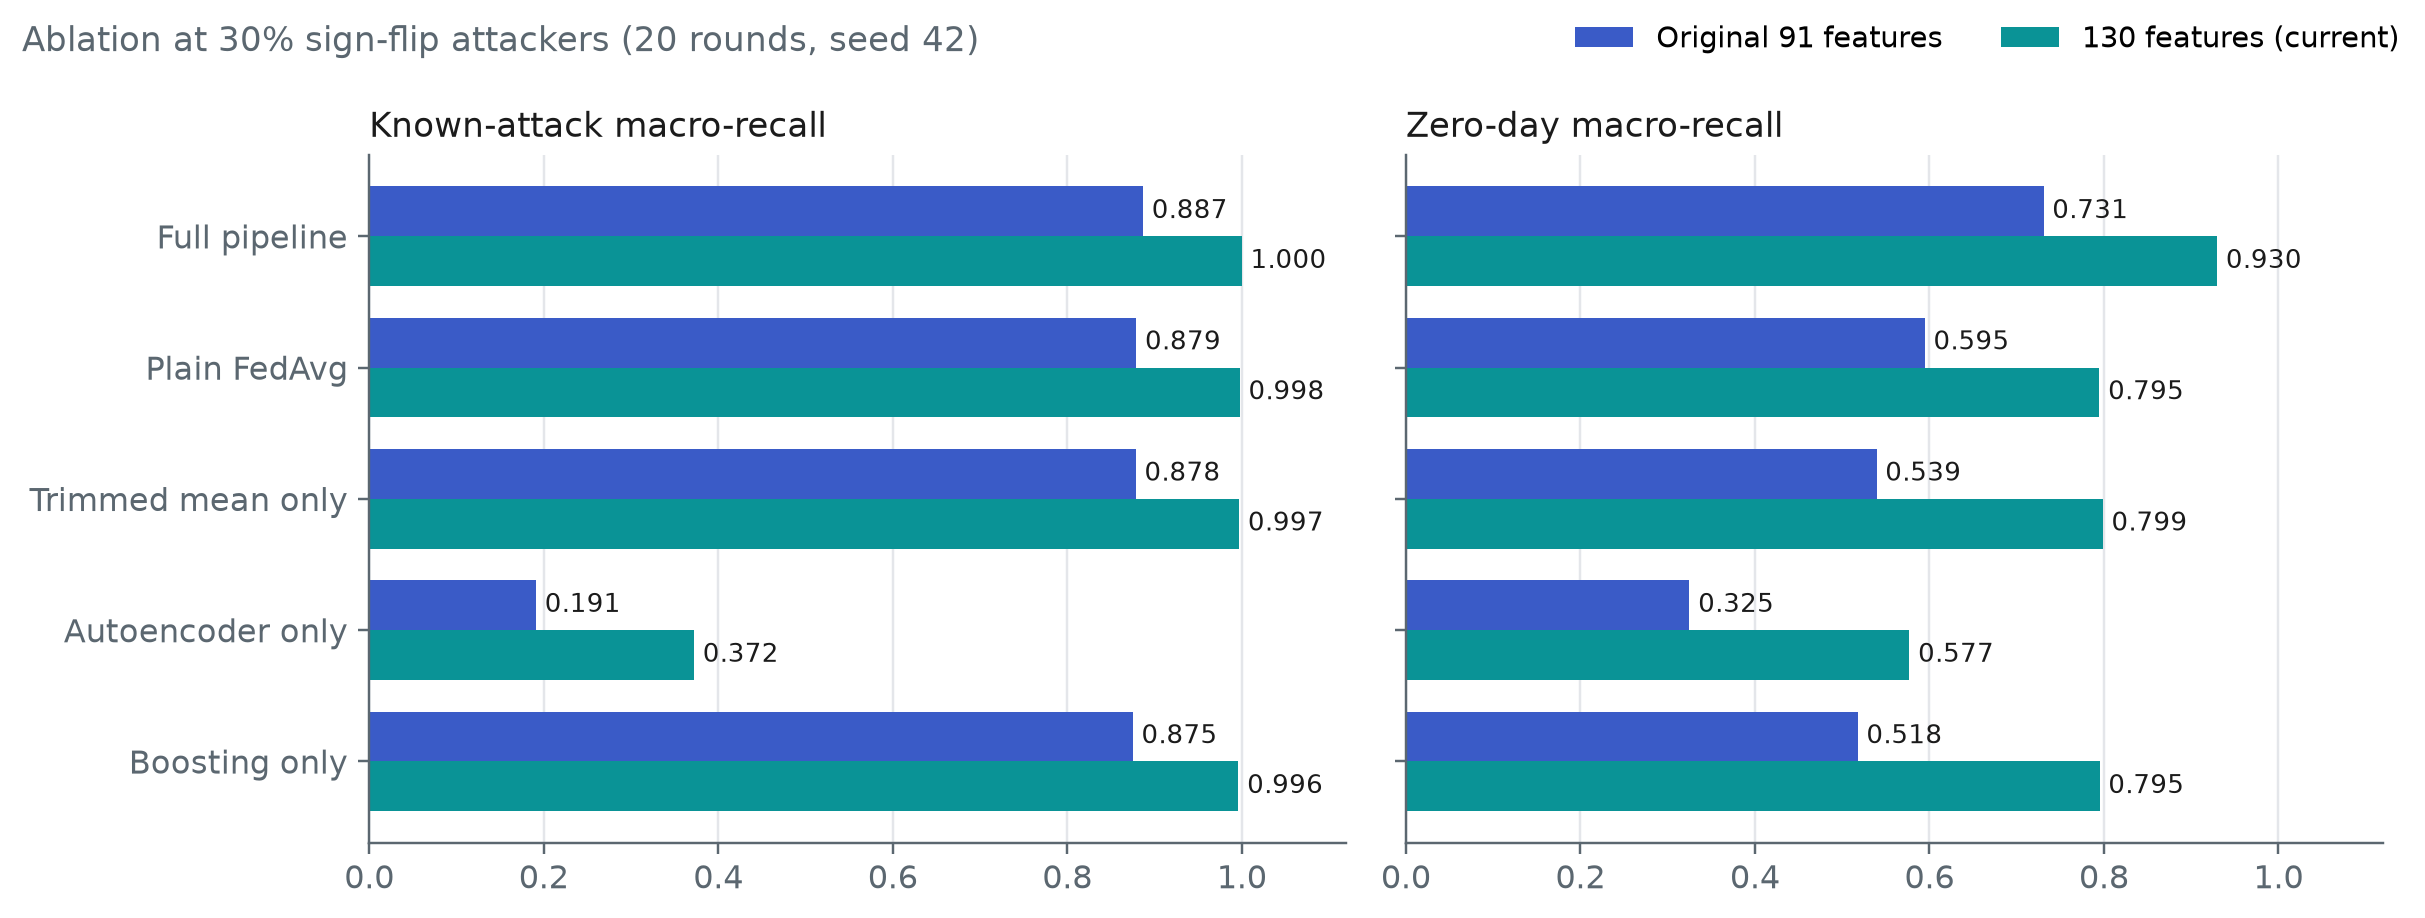
\includegraphics[width=\linewidth]{figures/ablation.png}
\caption{Ablation: known-attack and zero-day macro-recall, original vs.\ current features}
\label{fig:ablation}
\end{figure}
One trade-off is worth stating. On known attacks, boosting alone now has a higher detection F1 than the full cascade (0.998 vs.\ 0.961). The autoencoder's threshold is set to flag about 3\% of benign traffic, and that cost now outweighs the little it adds when the classifier already catches 99.6\% of known attacks. Final validation losses: full pipeline 0.028; plain FedAvg $5.0\times10^{20}$ and trimmed mean $1.3\times10^{4}$ (diverged). Communication: 15.7\,MB over 20 rounds (the autoencoder now has 9{,}834 parameters, up from 7{,}299).

\section{Poisoning resistance}
Figure~\ref{fig:poison} sweeps the share of sign-flip attackers from 0 to 50\%. Attack macro-recall stays between 0.997 and 1.000 at every fraction [0.878--0.887], and zero-day macro-recall between 0.901 and 0.943 up to 40\% [0.724--0.736]. Attackers got past the filter in 10\%, 12\% and 36\% of attacker-rounds at 20\%, 30\% and 40\% [28\%, 32\%, 24\%]: lower at the first two fractions but higher at 40\%, although the autoencoder still held there (stand-alone recall 0.691). At 50\% the coordinate-wise median reference becomes the attackers' direction again: every attacker update passes, the autoencoder collapses, and zero-day detection falls back to the classifier (0.803). This is the known limit of median-based defences~\cite{yin2018trimmed}. A repeat with seeds 43 and 44 at 20\% and 30\% gave 0.996--0.999 attack macro-recall for every seed, while stand-alone autoencoder recall varied by seed (0.56--0.74), as it did with the original features.
\begin{figure}[H]
\centering
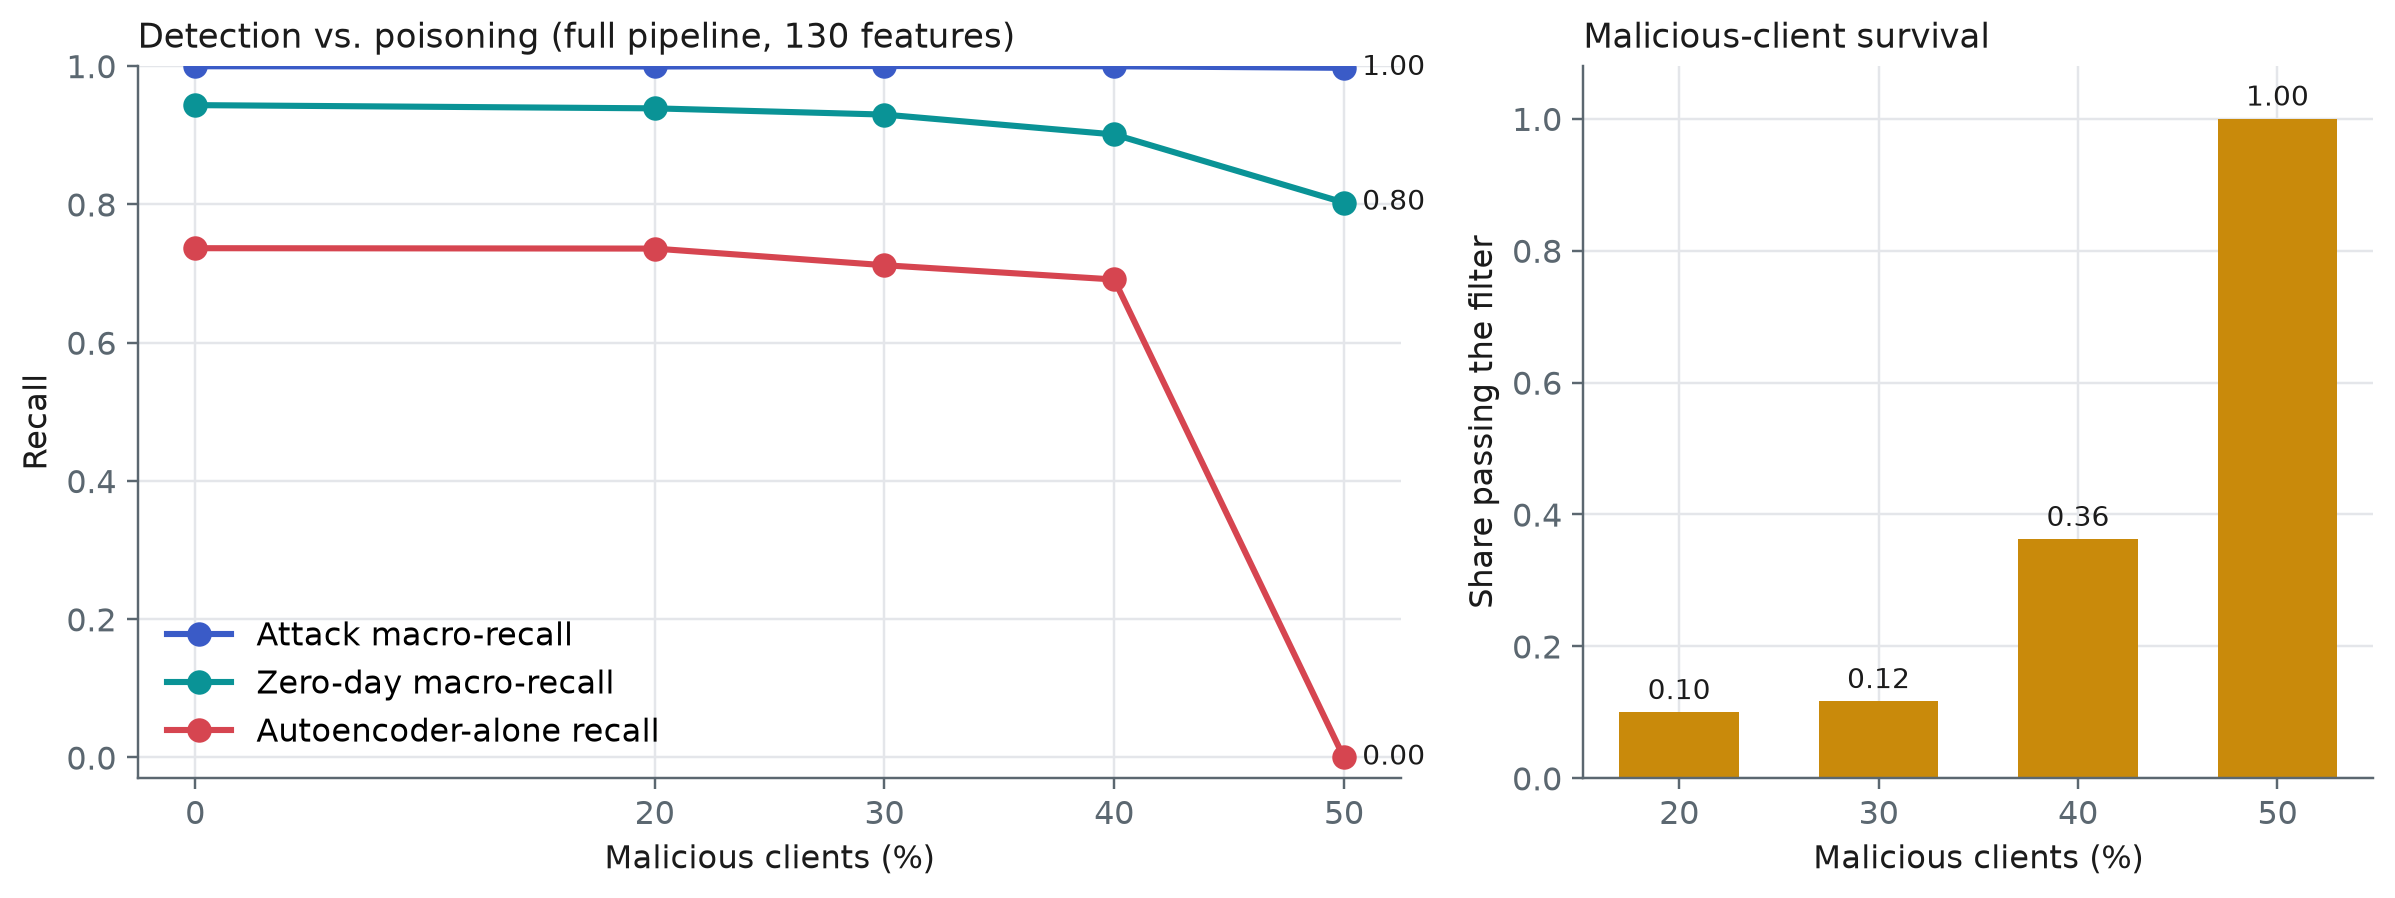
\includegraphics[width=\linewidth]{figures/poisoning_sweep.png}
\caption{Detection and malicious-client survival vs.\ share of malicious clients (130 features)}
\label{fig:poison}
\end{figure}

\section{Zero-day detection}
Each of the 14 attack classes was removed in turn from all training data (including scaler statistics) and then scored as unseen traffic (Figures~\ref{fig:zeroday} and~\ref{fig:zerodaycmp}). The cascade's average detection rose from 0.736 to \textbf{0.943}; boosting alone from 0.533 to 0.801 and the autoencoder alone from 0.493 to 0.757. The autoencoder separates unseen attacks from benign traffic far better than before (AUROC 0.968--1.000 for every class, against 0.59--0.70 for the HTTP-family attacks with the original features). The largest gains are on the attacks that were hardest before: Password 0.44$\rightarrow$0.97, Ransomware 0.54$\rightarrow$1.00, SQL\_injection 0.61$\rightarrow$1.00, XSS 0.52$\rightarrow$0.99 and DDoS\_HTTP 0.36$\rightarrow$0.88.

Two classes got worse and are reported rather than hidden. MITM fell from 0.89 to 0.69: its single ARP connection gets ordinary-looking connection features, so the autoencoder finds it less unusual. Unseen Uploading traffic now looks normal to the classifier (boosting-only 0.49$\rightarrow$0.08); the autoencoder catches most of it, so the cascade still improves (0.52$\rightarrow$0.72). The benign false-positive rate stays about 3\%, as set by the 97th-percentile threshold.
\begin{figure}[H]
\centering
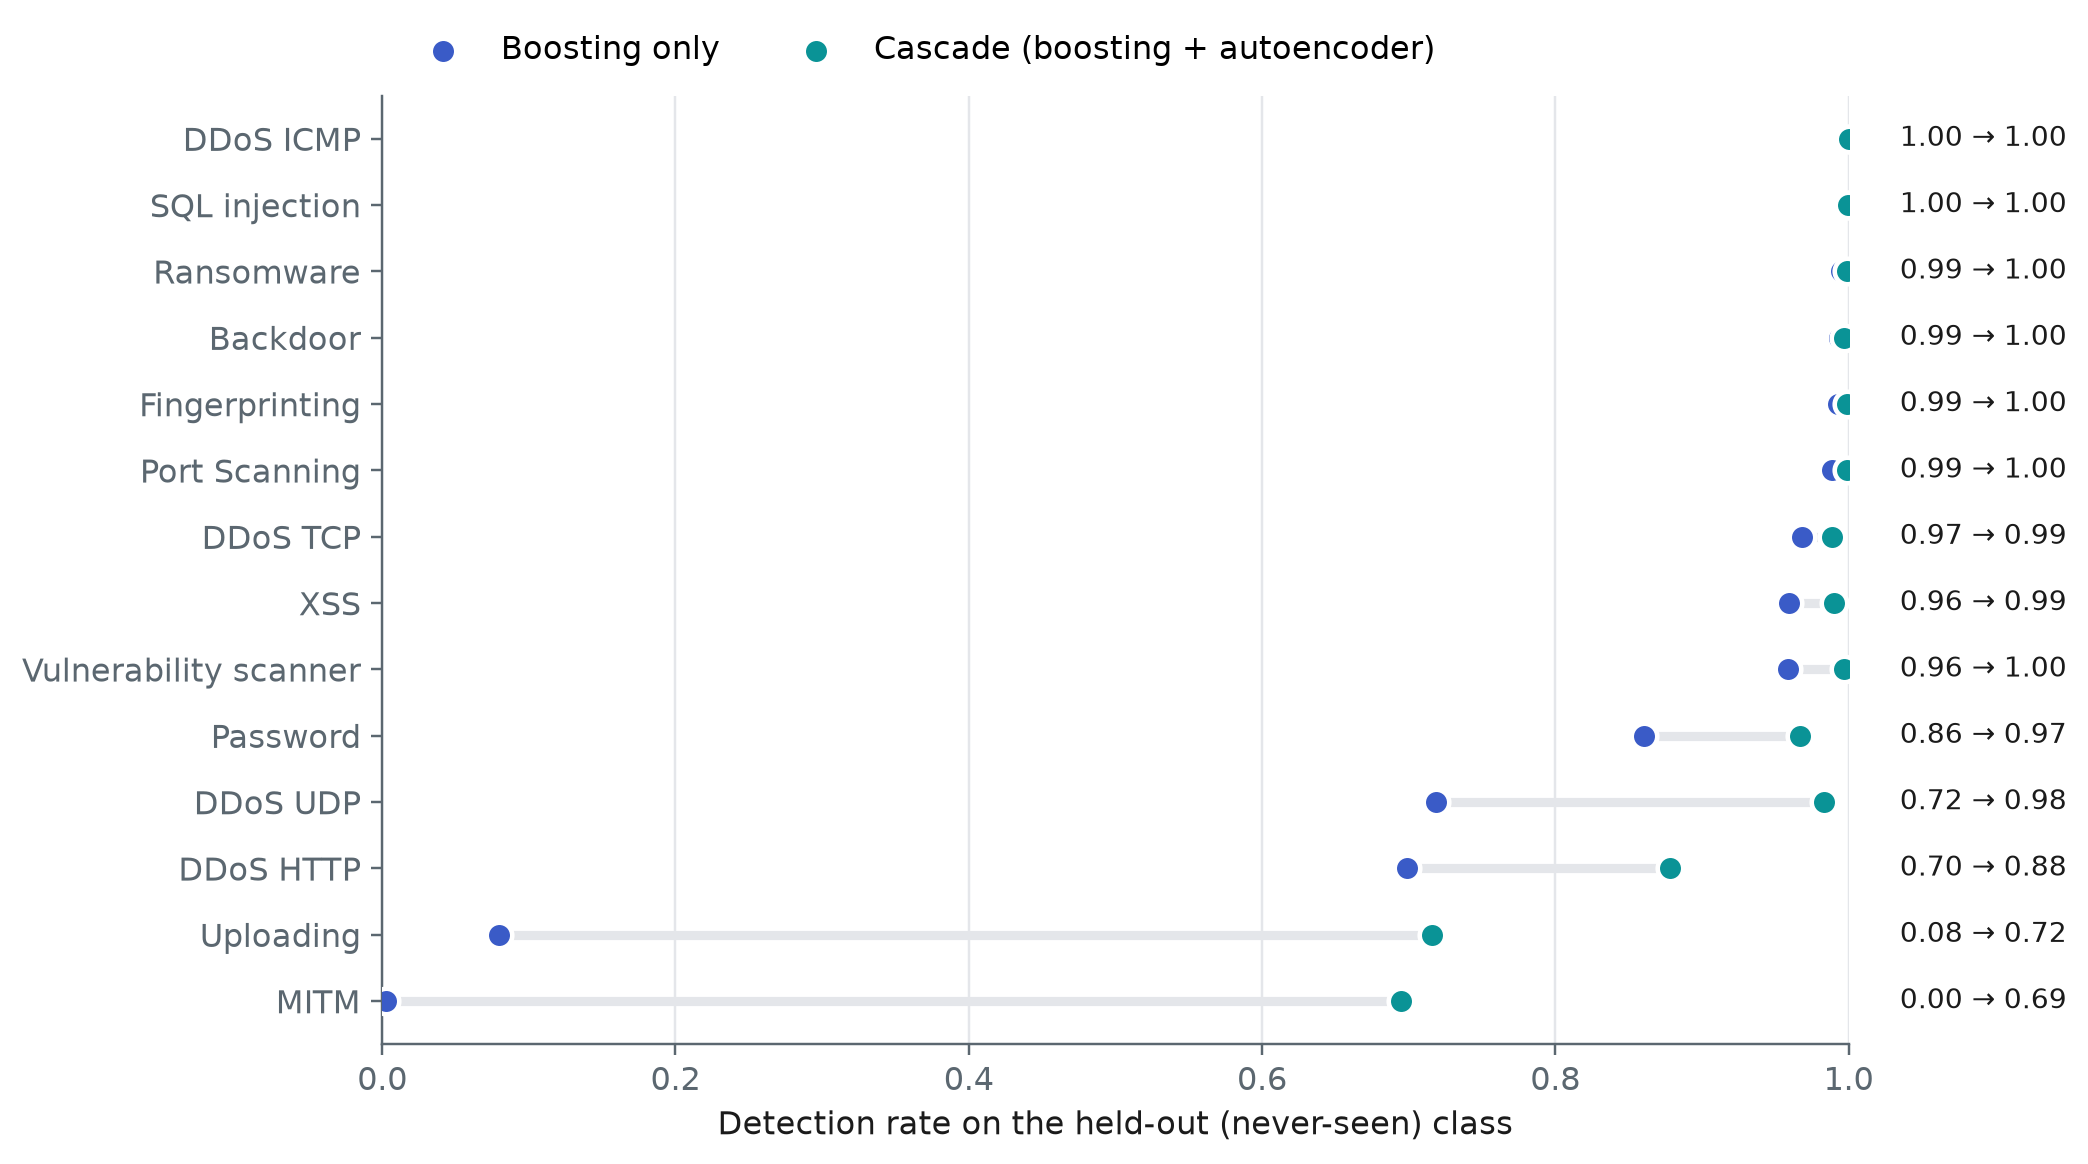
\includegraphics[width=0.88\linewidth]{figures/zero_day.png}
\caption{Zero-day detection per held-out class: boosting alone vs.\ cascade (130 features)}
\label{fig:zeroday}
\end{figure}
\begin{figure}[H]
\centering
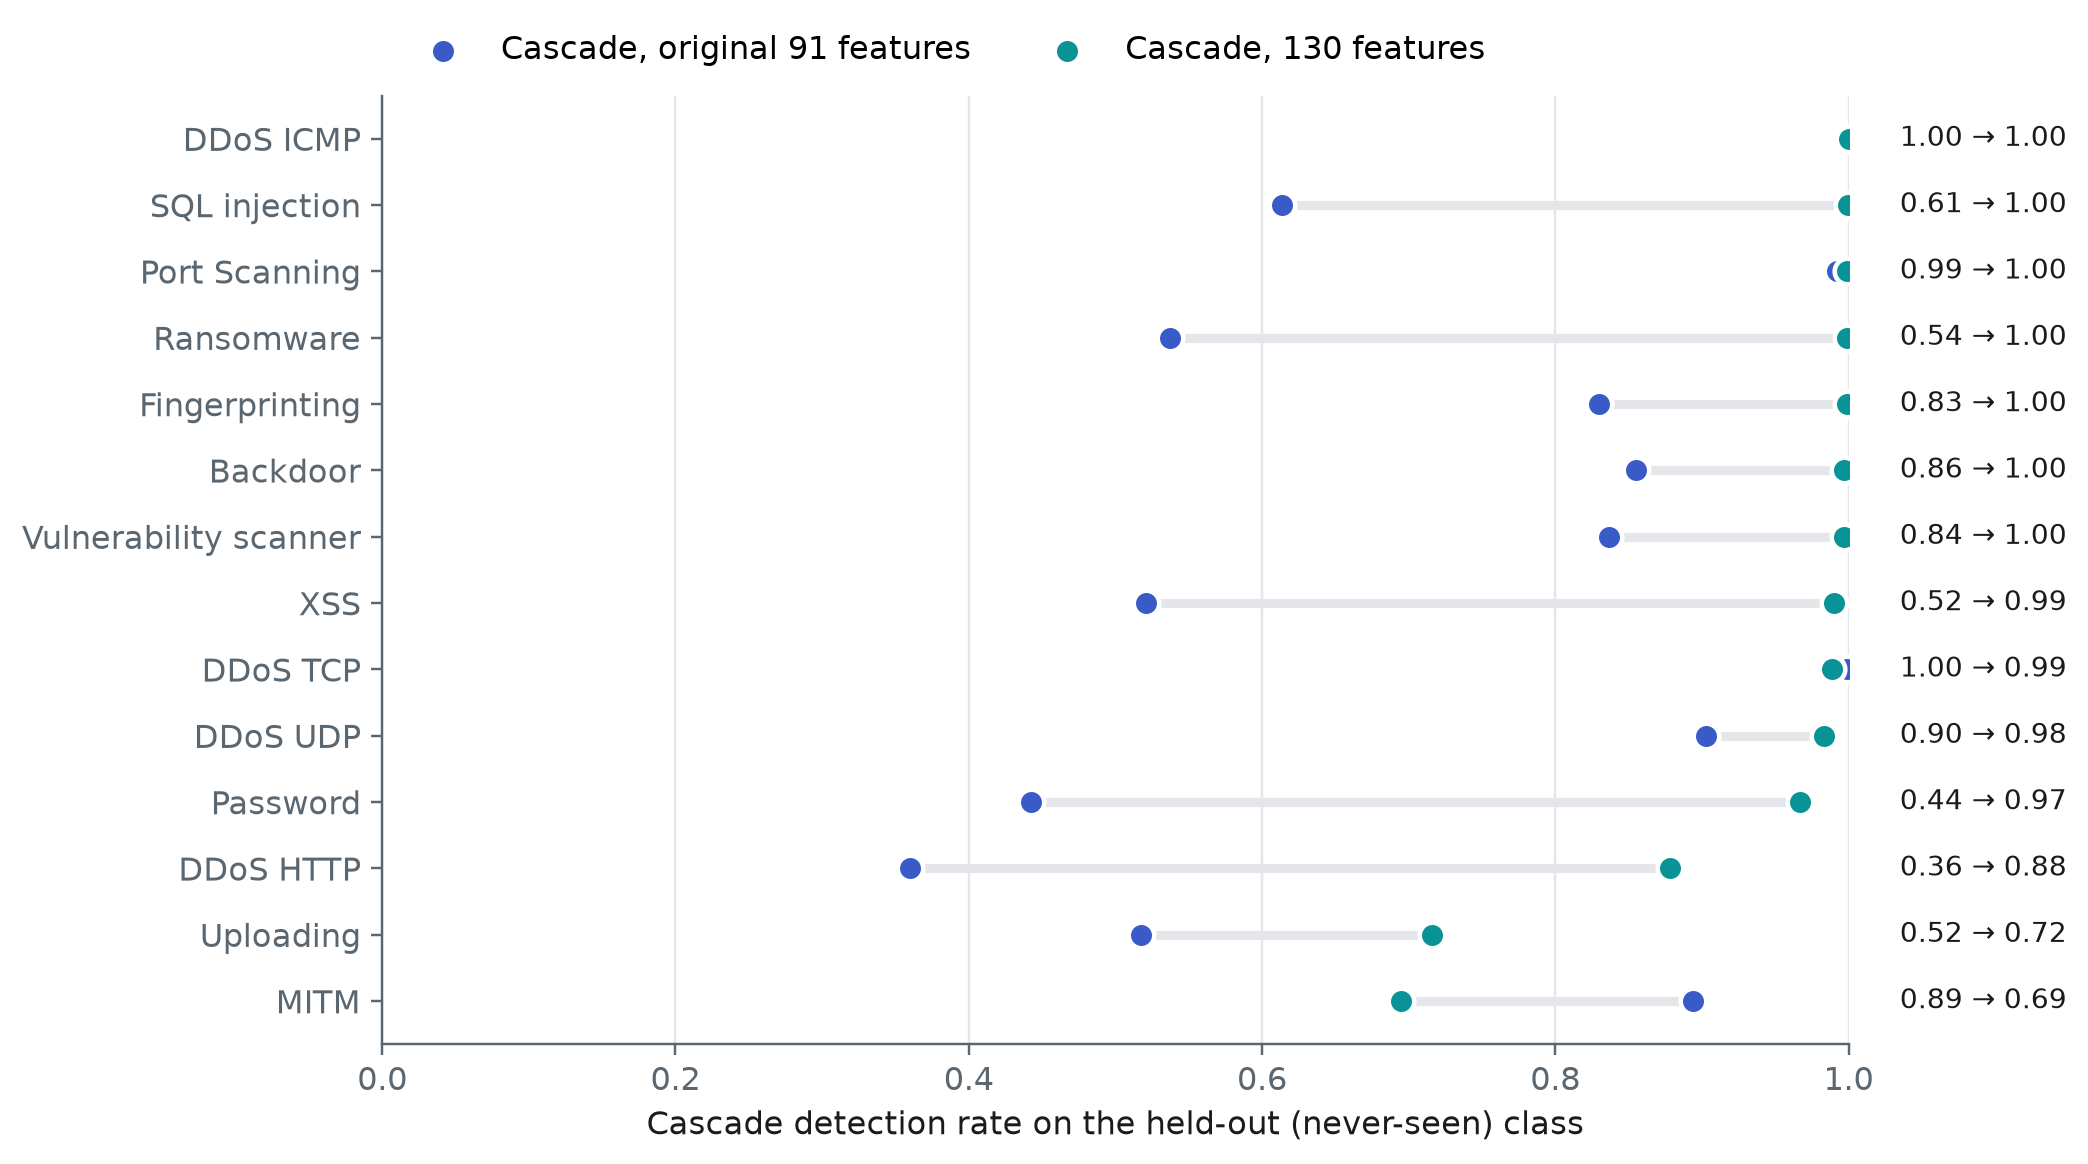
\includegraphics[width=0.88\linewidth]{figures/zero_day_compare.png}
\caption{Cascade zero-day detection per held-out class: original 91 features vs.\ 130 features}
\label{fig:zerodaycmp}
\end{figure}

\section{Real multi-process run and SDN mitigation}
\textbf{Phase A, real run.} A real Flower server and 10 separate client processes completed 20 rounds in about 4 minutes. The bootstrap classifier reached 0.997 accuracy on the calibration hold-out [0.963]. The final cascade gave \textbf{0.999} attack macro-recall [0.889] and a 0.035 benign false-positive rate [0.035] on the clients' test slices. A separate full-pipeline run scored per class gave 0.976 accuracy and 0.971 macro F1 for the cascade [0.944 / 0.931], and an autoencoder AUROC of 0.982 [0.805].

\textbf{Phase B.} Live extraction now derives the same 130 features from the capture with the same code as training: for \texttt{Backdoor\_attack.pcap}, 99.8\% of the live rows are identical to that capture's training rows. Replayed through Mininet with the new bundle, the capture was classified as \textbf{Backdoor with 0.997 confidence} by the boosting stage, 24{,}669 of its 24{,}914 packets were flagged [23{,}895], the bridge chose \emph{block}, and the rule \texttt{priority=100,ip,nw\_src=10.0.0.1 actions=drop} was confirmed in the switch's flow table. Because classification happens once features have been extracted from the whole capture, 23{,}161 replayed packets had already been forwarded when the rule appeared. The mitigation is therefore capture-level, not inline per-packet blocking.

\section{Scaling to 20 clients, repeat seeds and run timing}
\textbf{Real 20-process runs.} The project was re-hosted on a virtual machine with 24~GB of memory, which can hold one Flower server and 20 client processes (an earlier attempt on a 7.4~GB machine could not). Phase A was run with 10 and with 20 real client processes at seeds 42, 43 and 44 (20 rounds, no attackers). The seed changes the data split, the Dirichlet partition and the initialisation. Table~\ref{tab:realruns} lists every run. Over the three seeds the cascade's attack macro-recall averages 0.998 with 10 clients and 0.992 with 20 clients, and the benign false-positive rate stays between 2.8\% and 4.0\%. At seed 42, the 20-client run dips to 0.978; this run was not analysed per class, so its cause is not established. With only three seeds, no confidence intervals are claimed.

\begin{table}[H]
\centering
\renewcommand{\arraystretch}{1.2}
\begin{tabular}{|l|c|c|c|c|}
\hline
\textbf{Run} & \textbf{Phase A (s)} & \textbf{Attack macro-recall} & \textbf{False alarms} & \textbf{Classifier acc.} \\ \hline
10 clients, seed 42 & 341 & 0.999 & 3.40\% & 0.9969 \\ \hline
10 clients, seed 43 & 276 & 0.999 & 3.11\% & 0.9976 \\ \hline
10 clients, seed 44 & 262 & 0.996 & 2.84\% & 0.9968 \\ \hline
20 clients, seed 42 & 247 & 0.978 & 3.62\% & 0.9969 \\ \hline
20 clients, seed 43 & 238 & 0.999 & 2.84\% & 0.9976 \\ \hline
20 clients, seed 44 & 242 & 0.999 & 3.96\% & 0.9968 \\ \hline
\end{tabular}
\caption{Real multi-process Phase A runs (source: \texttt{results/real\_runs/summary.md})}
\label{tab:realruns}
\end{table}

Phase B on the 20-client bundle classified \texttt{Backdoor\_attack.pcap} as Backdoor with 0.997 confidence, flagged 24{,}466 of 24{,}914 packets, and the drop rule \texttt{priority=100,ip,nw\_src=10.0.0.1 actions=drop} was read back from the switch.

\textbf{The trust filter without attackers.} Even with no malicious clients, the filter excluded some clients' updates: over 20 rounds, 15, 2 and 6 client-rounds with 10 clients, and 38, 42 and 27 with 20 clients (seeds 42, 43, 44). These are honest clients whose non-IID updates look unlike the median, so the filter cannot tell unusual data from sabotage. This is the confound named in the limitations, and it is more frequent with 20 clients.

\textbf{Simulation versus real run.} An in-process simulation of 20 clients (seed 42) gave a cascade attack-detection recall of 0.9960 against 0.9996 for 10 clients, an autoencoder recall of 0.685 against 0.728, and benign false alarms of 3.72\% against 3.32\%. Three of the 20 simulated clients received no benign validation rows, so their anomaly threshold is infinite and their autoencoder never flags. The simulation uses the same client, strategy and trust-filter code as the real run, and the table above is the real-process evidence.

\textbf{Timing of one complete run.} One real run (10 client processes, warm feature cache) took 219~s in total: Phase A 210.6~s, of which federated training was 191.2~s, and Phase B 8.6~s. Tables~\ref{tab:timea} and~\ref{tab:timeb} give the stages.

\begin{table}[H]
\centering
\renewcommand{\arraystretch}{1.2}
\begin{tabular}{|l|c|}
\hline
\textbf{Phase A stage} & \textbf{Seconds} \\ \hline
Load, clean and encode the dataset & 1.9 \\ \hline
Calibration split, bootstrap classifier, client partition & 14.4 \\ \hline
Federated training & 191.2 \\ \hline
Calibrate client anomaly thresholds & 0.1 \\ \hline
Evaluate on the clients' test slices & 2.5 \\ \hline
Save the model bundle & 0.2 \\ \hline
\end{tabular}
\caption{Phase A stage timing (source: \texttt{results/journey/phase\_a\_journey.json})}
\label{tab:timea}
\end{table}

\begin{table}[H]
\centering
\renewcommand{\arraystretch}{1.2}
\begin{tabular}{|l|c|}
\hline
\textbf{Phase B stage} & \textbf{Seconds} \\ \hline
Load the model bundle & 0.08 \\ \hline
Start the SDN bridge and controller & 2.20 \\ \hline
Network, replay, classify and block (root process) & 6.33 \\ \hline
Check the switch's flow table & 0.00 \\ \hline
\end{tabular}
\caption{Phase B stage timing (source: \texttt{results/journey/phase\_b\_journey.json})}
\label{tab:timeb}
\end{table}

\section{Follow-up experiments: more seeds, an adaptive attacker, pruning and a time-ordered split}\label{sec:followups}
These experiments were run after the main results, in the virtual machine, and every table is generated from the experiments' own result files.

\textbf{More seeds.} The ablation, the poisoning sweep and the zero-day experiment were repeated at seeds 43 and 44 (Tables~\ref{tab:fu_seed_ablation}--\ref{tab:fu_seed_zeroday}). The conclusions hold in all three seeds: the full pipeline's attack macro-recall stays between 0.995 and 1.000 up to 50\% attackers; plain FedAvg and the trimmed mean alone leave the autoencoder at recall 0.000--0.026 with 30\% attackers; the trust filter fails at 50\% (attacker survival 0.97--1.00); and the cascade's mean zero-day detection is 0.943, 0.952 and 0.952. Other numbers move with the seed: the autoencoder's recall at 30\% attackers ranges from 0.565 to 0.712, attacker survival at 20\% from 0.03 to 0.23, and MITM zero-day detection from 0.695 to 0.963. The per-class zero-day columns inside the ablation and sweep tables were not repeated at seeds 43 and 44 (about 85 extra trainings per seed). Three seeds are too few for confidence intervals.

\begin{table}[H]
\centering
\small
\setlength{\tabcolsep}{3pt}
\renewcommand{\arraystretch}{1.15}
\begin{tabular}{|l|c|c|c|}
\hline
\textbf{Variant} & \textbf{Attack macro-recall} & \textbf{Autoencoder-alone recall} & \textbf{Benign FPR} \\ \hline
full\_pipeline & 1.000 / 0.999 / 0.997 & 0.712 / 0.679 / 0.565 & 0.0309 / 0.0284 / 0.0320 \\ \hline
plain\_fedavg & 0.998 / 0.997 / 0.994 & 0.002 / 0.000 / 0.000 & 0.0347 / 0.0317 / 0.0297 \\ \hline
trimmed\_mean\_only & 0.997 / 0.997 / 0.996 & 0.000 / 0.000 / 0.026 & 0.0334 / 0.0291 / 0.0337 \\ \hline
autoencoder\_only & 0.372 / 0.295 / 0.306 & 0.372 / 0.295 / 0.306 & 0.0301 / 0.0281 / 0.0325 \\ \hline
boosting\_only & 0.996 / 0.997 / 0.996 & n/a / n/a / n/a & 0.0002 / 0.0000 / 0.0005 \\ \hline
\end{tabular}
\caption{Ablation at 30\% sign-flip attackers, seeds 42 / 43 / 44 (source: results/seeds/summary.json)}
\label{tab:fu_seed_ablation}
\end{table}
\begin{table}[H]
\centering
\small
\setlength{\tabcolsep}{3pt}
\renewcommand{\arraystretch}{1.15}
\begin{tabular}{|l|c|c|c|}
\hline
\textbf{Attackers} & \textbf{Attack macro-recall} & \textbf{Autoencoder-alone recall} & \textbf{Attacker survival} \\ \hline
0\% & 1.000 / 0.999 / 0.997 & 0.737 / 0.765 / 0.612 & n/a / n/a / n/a \\ \hline
20\% & 0.999 / 0.999 / 0.996 & 0.736 / 0.739 / 0.618 & 0.10 / 0.03 / 0.23 \\ \hline
30\% & 1.000 / 0.999 / 0.997 & 0.712 / 0.679 / 0.565 & 0.12 / 0.12 / 0.27 \\ \hline
40\% & 1.000 / 0.998 / 0.997 & 0.691 / 0.620 / 0.537 & 0.36 / 0.31 / 0.44 \\ \hline
50\% & 0.997 / 0.997 / 0.995 & 0.000 / 0.000 / 0.000 & 1.00 / 0.99 / 0.97 \\ \hline
\end{tabular}
\caption{Poisoning sweep, seeds 42 / 43 / 44}
\label{tab:fu_seed_sweep}
\end{table}
\begin{table}[H]
\centering
\small
\setlength{\tabcolsep}{3pt}
\renewcommand{\arraystretch}{1.15}
\begin{tabular}{|l|c|}
\hline
\textbf{Stage} & \textbf{Mean detection rate} \\ \hline
Classifier alone & 0.801 / 0.748 / 0.791 \\ \hline
Autoencoder alone & 0.757 / 0.775 / 0.747 \\ \hline
Cascade & 0.943 / 0.952 / 0.952 \\ \hline
Cascade, DDoS\_HTTP & 0.878 / 0.846 / 0.948 \\ \hline
Cascade, MITM & 0.695 / 0.963 / 0.837 \\ \hline
Cascade, Uploading & 0.716 / 0.677 / 0.665 \\ \hline
\end{tabular}
\caption{Zero-day detection of the unseen class, mean over 14 classes, seeds 42 / 43 / 44}
\label{tab:fu_seed_zeroday}
\end{table}
\textbf{Why the 20-client run dipped.} The seed-42 run with 20 real clients scored attack macro-recall 0.978, against 0.996--0.999 elsewhere. The cause is one missed Fingerprinting test row out of four; micro recall is 0.9964 (Table~\ref{tab:fu_realrun_breakdown}). Clients without benign validation rows (infinite threshold) were still caught by the classifier.

\begin{table}[H]
\centering
\scriptsize
\setlength{\tabcolsep}{3pt}
\renewcommand{\arraystretch}{1.15}
\begin{tabular}{|l|c|c|c|c|c|}
\hline
\textbf{Run} & \textbf{Macro-recall} & \textbf{Micro recall} & \textbf{Fingerprinting test rows, recall} & \textbf{MITM test rows, recall} & \textbf{Clients with infinite threshold} \\ \hline
10 clients, seed 42 & 0.999 & 0.9992 & 3 rows, 1.00 & 3 rows, 1.00 & 0 \\ \hline
10 clients, seed 43 & 0.999 & 0.9992 & 4 rows, 1.00 & 4 rows, 1.00 & 1 \\ \hline
10 clients, seed 44 & 0.996 & 0.9960 & 4 rows, 1.00 & 5 rows, 1.00 & 1 \\ \hline
20 clients, seed 42 & 0.978 & 0.9964 & 4 rows, 0.75 & 1 rows, 1.00 & 3 \\ \hline
20 clients, seed 43 & 0.999 & 0.9992 & 2 rows, 1.00 & 3 rows, 1.00 & 2 \\ \hline
20 clients, seed 44 & 0.999 & 0.9988 & 2 rows, 1.00 & 3 rows, 1.00 & 2 \\ \hline
\end{tabular}
\caption{Where the real-run macro-recall comes from (source: results/real\_runs/<run>/, made by fl\_ids.eval.bundle\_report)}
\label{tab:fu_realrun_breakdown}
\end{table}
\textbf{Real attackers.} With sign-flip attackers in the real multi-process run, the trust filter excluded the attackers' updates in 36 of 40 (20\%) and 52 of 60 (30\%) client-rounds, and excluded no honest client (Table~\ref{tab:fu_attack_runs}, Figure~\ref{fig:trustmal03}).

\begin{table}[H]
\centering
\scriptsize
\setlength{\tabcolsep}{3pt}
\renewcommand{\arraystretch}{1.15}
\begin{tabular}{|l|c|c|c|c|c|}
\hline
\textbf{Attackers} & \textbf{Attacker clients} & \textbf{Attacker client-rounds excluded} & \textbf{Honest client-rounds excluded} & \textbf{Attack macro-recall} & \textbf{Benign FPR} \\ \hline
20\% & 0,7 & 36 of 40 & 0 of 160 & 0.998 & 0.0335 \\ \hline
30\% & 0,6,9 & 52 of 60 & 0 of 140 & 0.999 & 0.0317 \\ \hline
\end{tabular}
\caption{Real multi-process Phase A with sign-flip attackers (10 clients, 20 rounds, seed 42; source: runs/attack\_runs/)}
\label{tab:fu_attack_runs}
\end{table}
\begin{figure}[H]
\centering
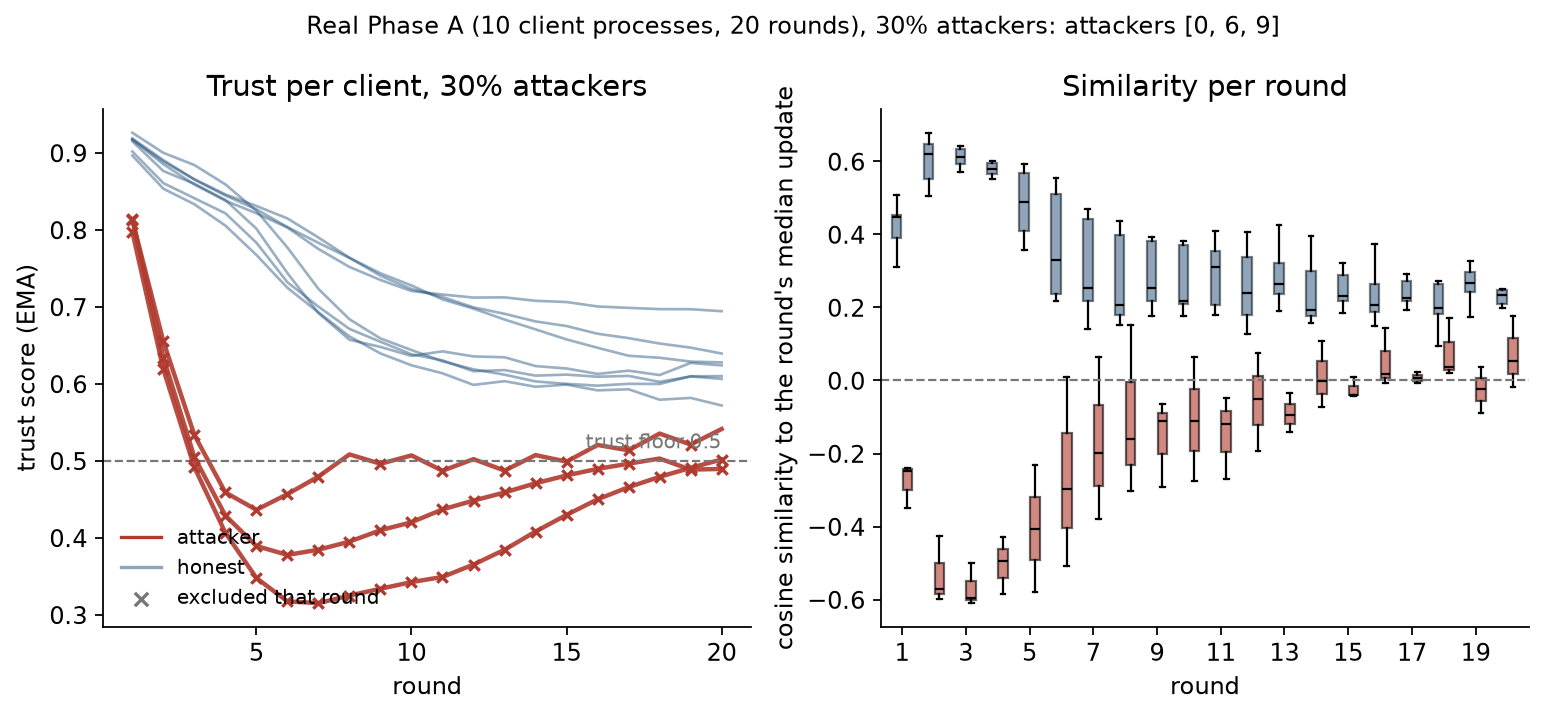
\includegraphics[width=0.98\linewidth]{figures/trust_mal03.png}
\caption{Real run with 30\% sign-flip attackers: trust score (left) and cosine similarity to the round's median update (right)}
\label{fig:trustmal03}
\end{figure}
\textbf{An adaptive attacker.} A white-box attacker that knows the filter's rule estimates the consensus from the last aggregate update, keeps a cosine similarity of 0.1 to it, and spends the rest of a norm budget (1.5 times its honest norm, under the clip) on the opposite of its honest update's orthogonal component. The filter mostly fails against it: attackers survive in 72--90\% of client-rounds instead of 10--36\% (Table~\ref{tab:fu_adaptive}). The damage is bounded: known-attack recall stays at 0.9997 or above, but the autoencoder's recall alone falls to 0.499 at 40\% attackers (0.663 for sign-flip). Zero-day detection under this attacker was not measured, and this is one adaptive strategy, not a proof for all.

\begin{table}[H]
\centering
\scriptsize
\setlength{\tabcolsep}{3pt}
\renewcommand{\arraystretch}{1.15}
\begin{tabular}{|l|c|c|c|c|c|}
\hline
\textbf{Attack} & \textbf{Attackers} & \textbf{Attack macro-recall} & \textbf{Autoencoder-alone recall} & \textbf{Attacker survival} & \textbf{Final validation loss} \\ \hline
sign\_flip & 20\% & 0.9993 & 0.730 & 0.10 & 0.026 \\ \hline
sign\_flip & 30\% & 1.0000 & 0.718 & 0.12 & 0.029 \\ \hline
sign\_flip & 40\% & 0.9997 & 0.663 & 0.36 & 0.021 \\ \hline
stealth & 20\% & 0.9997 & 0.747 & 0.90 & 0.041 \\ \hline
stealth & 30\% & 1.0000 & 0.741 & 0.72 & 0.040 \\ \hline
stealth & 40\% & 0.9997 & 0.499 & 0.82 & 0.037 \\ \hline
\end{tabular}
\caption{Adaptive (stealth) attacker vs. sign-flip, seed 42, 20 rounds (source: results/adaptive/adaptive\_attack.csv)}
\label{tab:fu_adaptive}
\end{table}
\textbf{Weight pruning (Objective 3).} The autoencoder's weight matrices were magnitude-pruned after training and during federated training (the server re-prunes every round). Pruning after training damages the backstop at once, while pruning during training keeps it up to about 70\% sparsity: autoencoder-alone recall 0.744 dense, 0.727 at 50\%, 0.688 at 70\%, then 0.467 at 80\% (Tables~\ref{tab:fu_prune_post} and~\ref{tab:fu_prune_fl}). A sparse layout needs index storage, so the size falls below the dense size only past 50\% sparsity (0.61 of the dense bytes at 70\%; computed from the non-zero counts, not transmitted). Clients still send dense updates, so this reduces the model, not the per-round communication. Single seed, no attackers.

\begin{table}[H]
\centering
\scriptsize
\setlength{\tabcolsep}{3pt}
\renewcommand{\arraystretch}{1.15}
\begin{tabular}{|l|c|c|c|c|c|c|}
\hline
\textbf{Sparsity} & \textbf{Non-zero weights} & \textbf{Sparse / dense bytes} & \textbf{Autoencoder recall} & \textbf{Autoencoder AUROC} & \textbf{Cascade macro-recall} & \textbf{Benign FPR} \\ \hline
0\% & 9600 & 1.98 & 0.742 & 0.987 & 0.999 & 0.0340 \\ \hline
50\% & 4800 & 1.00 & 0.273 & 0.742 & 0.998 & 0.0287 \\ \hline
70\% & 2880 & 0.61 & 0.168 & 0.596 & 0.998 & 0.0292 \\ \hline
80\% & 1920 & 0.41 & 0.145 & 0.559 & 0.996 & 0.0334 \\ \hline
90\% & 960 & 0.22 & 0.144 & 0.594 & 0.996 & 0.0323 \\ \hline
95\% & 480 & 0.12 & 0.147 & 0.593 & 0.996 & 0.0366 \\ \hline
98\% & 192 & 0.06 & 0.147 & 0.593 & 0.996 & 0.0366 \\ \hline
\end{tabular}
\caption{Post-training magnitude pruning of the 10-client autoencoder, thresholds recalibrated (source: results/pruning/c10\_s42/pruning.csv)}
\label{tab:fu_prune_post}
\end{table}
\begin{table}[H]
\centering
\scriptsize
\setlength{\tabcolsep}{3pt}
\renewcommand{\arraystretch}{1.15}
\begin{tabular}{|l|c|c|c|c|c|c|}
\hline
\textbf{Sparsity} & \textbf{Non-zero weights} & \textbf{Sparse / dense bytes} & \textbf{Autoencoder-alone recall} & \textbf{Cascade macro-recall} & \textbf{Benign FPR} & \textbf{Final validation loss} \\ \hline
0\% & 9600 & 1.98 & 0.744 & 1.000 & 0.0320 & 0.034 \\ \hline
50\% & 4800 & 1.00 & 0.727 & 1.000 & 0.0323 & 0.040 \\ \hline
70\% & 2880 & 0.61 & 0.688 & 1.000 & 0.0298 & 0.049 \\ \hline
80\% & 1920 & 0.41 & 0.467 & 0.999 & 0.0312 & 0.080 \\ \hline
90\% & 960 & 0.22 & 0.176 & 0.998 & 0.0289 & 0.207 \\ \hline
\end{tabular}
\caption{Pruning during federated training (server re-prunes each round, linear ramp over the first 10 rounds), seed 42, no attackers (source: results/pruning/pruning\_during\_fl.csv)}
\label{tab:fu_prune_fl}
\end{table}
\textbf{Clipping.} Without the per-client z-score clip the benign validation loss stays near 50; with it, it falls from 0.2047 to 0.03369 (Table~\ref{tab:fu_clip}, Figure~\ref{fig:clipval}).

\begin{table}[H]
\centering
\scriptsize
\setlength{\tabcolsep}{3pt}
\renewcommand{\arraystretch}{1.15}
\begin{tabular}{|l|c|c|c|c|}
\hline
\textbf{Normalisation} & \textbf{Round 1} & \textbf{Round 5} & \textbf{Round 10} & \textbf{Round 20} \\ \hline
clip 10 & 0.2047 & 0.04336 & 0.03999 & 0.03369 \\ \hline
no clip & 50.63 & 50.15 & 50 & 49.86 \\ \hline
\end{tabular}
\caption{Benign validation loss with and without the per-client z-score clip (source: results/clip/clip\_comparison.csv)}
\label{tab:fu_clip}
\end{table}
\begin{figure}[H]
\centering
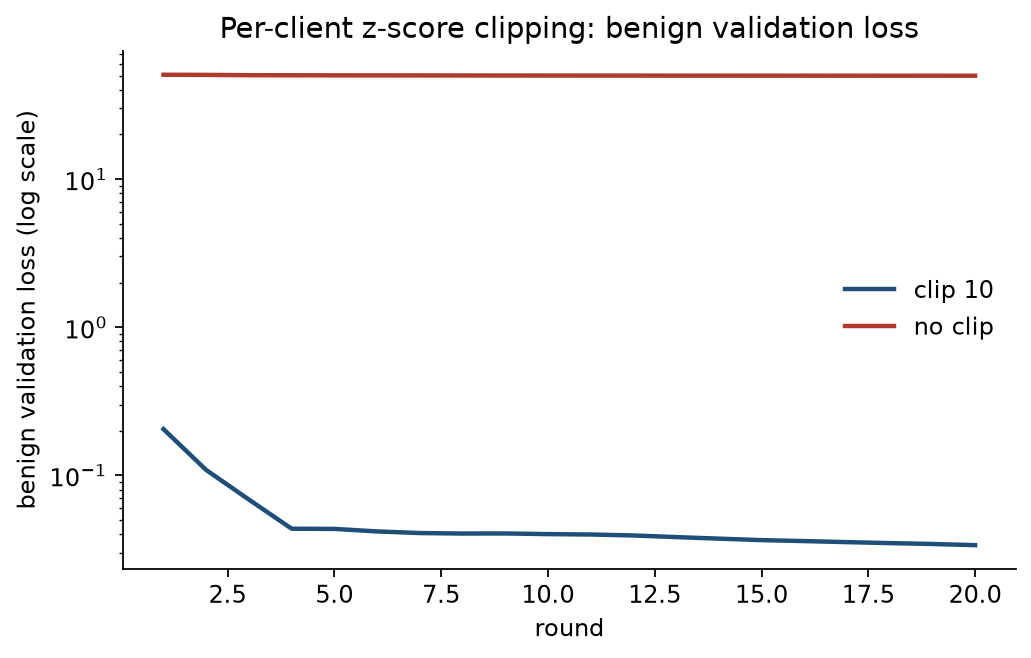
\includegraphics[width=0.7\linewidth]{figures/clip_val_loss.png}
\caption{Benign validation loss with and without the per-client z-score clip}
\label{fig:clipval}
\end{figure}
\textbf{A time-ordered split.} Each class's earliest 80\% of connections were used for training and its latest 20\% for testing (the CSV is in capture order within a class, but its timestamps carry no date, so this orders by row position). Accuracy is 0.994 against 0.997 for the connection-grouped split (Table~\ref{tab:fu_temporal_summary}). Macro F1 falls from 0.983 to 0.913, mostly because MITM is a single connection, so it falls entirely in the test side and enters the mean with recall 0; without it the figure is about 0.978. The real losses are Backdoor (0.989 to 0.947--0.962) and DDoS\_HTTP (0.980 to 0.912--0.925).

\begin{table}[H]
\centering
\small
\setlength{\tabcolsep}{3pt}
\renewcommand{\arraystretch}{1.15}
\begin{tabular}{|l|c|c|}
\hline
\textbf{Split} & \textbf{Accuracy} & \textbf{Macro F1} \\ \hline
Time-ordered, seeds 42 / 43 / 44 & 0.9942 / 0.9943 / 0.9941 & 0.9133 / 0.9122 / 0.9129 \\ \hline
Connection-grouped, seed 42 & 0.9972 & 0.9828 \\ \hline
\end{tabular}
\caption{Per-class time-ordered split vs. connection-grouped split (source: experiments/accuracy/results/full\_temporal\_bal\_s*.json)}
\label{tab:fu_temporal_summary}
\end{table}
\textbf{The placeholder leak, measured.} Before the fix, the four affected raw columns separate attack from normal with AUROC 0.9998--1.0. On the current 130-feature matrix the strongest single feature is the flow's reset count (0.879), followed by its packet count (0.866) and the service port (0.835); these are connection summaries rather than spelling artifacts (Table~\ref{tab:fu_leak}, Figure~\ref{fig:leakauroc}).

\begin{table}[H]
\centering
\small
\setlength{\tabcolsep}{3pt}
\renewcommand{\arraystretch}{1.15}
\begin{tabular}{|l|c|c|}
\hline
\textbf{Feature} & \textbf{AUROC} & \textbf{State} \\ \hline
mqtt.topic == 0.0 & 1.0000 & raw, before the fix \\ \hline
mqtt.conack.flags == 0.0 & 1.0000 & raw, before the fix \\ \hline
mqtt.protoname == 0.0 & 1.0000 & raw, before the fix \\ \hline
dns.qry.name.len == 0.0 & 0.9998 & raw, before the fix \\ \hline
f\_rst & 0.8789 & 130-feature matrix, after \\ \hline
f\_npkts & 0.8657 & 130-feature matrix, after \\ \hline
svc\_port & 0.8350 & 130-feature matrix, after \\ \hline
f\_fin & 0.8039 & 130-feature matrix, after \\ \hline
f\_pl\_nonzero & 0.7328 & 130-feature matrix, after \\ \hline
f\_syn & 0.7108 & 130-feature matrix, after \\ \hline
\end{tabular}
\caption{Single-feature AUROC, attack vs. normal (source: results/leak/single\_feature\_auroc.json; after: 300,000-row sample)}
\label{tab:fu_leak}
\end{table}
\begin{figure}[H]
\centering
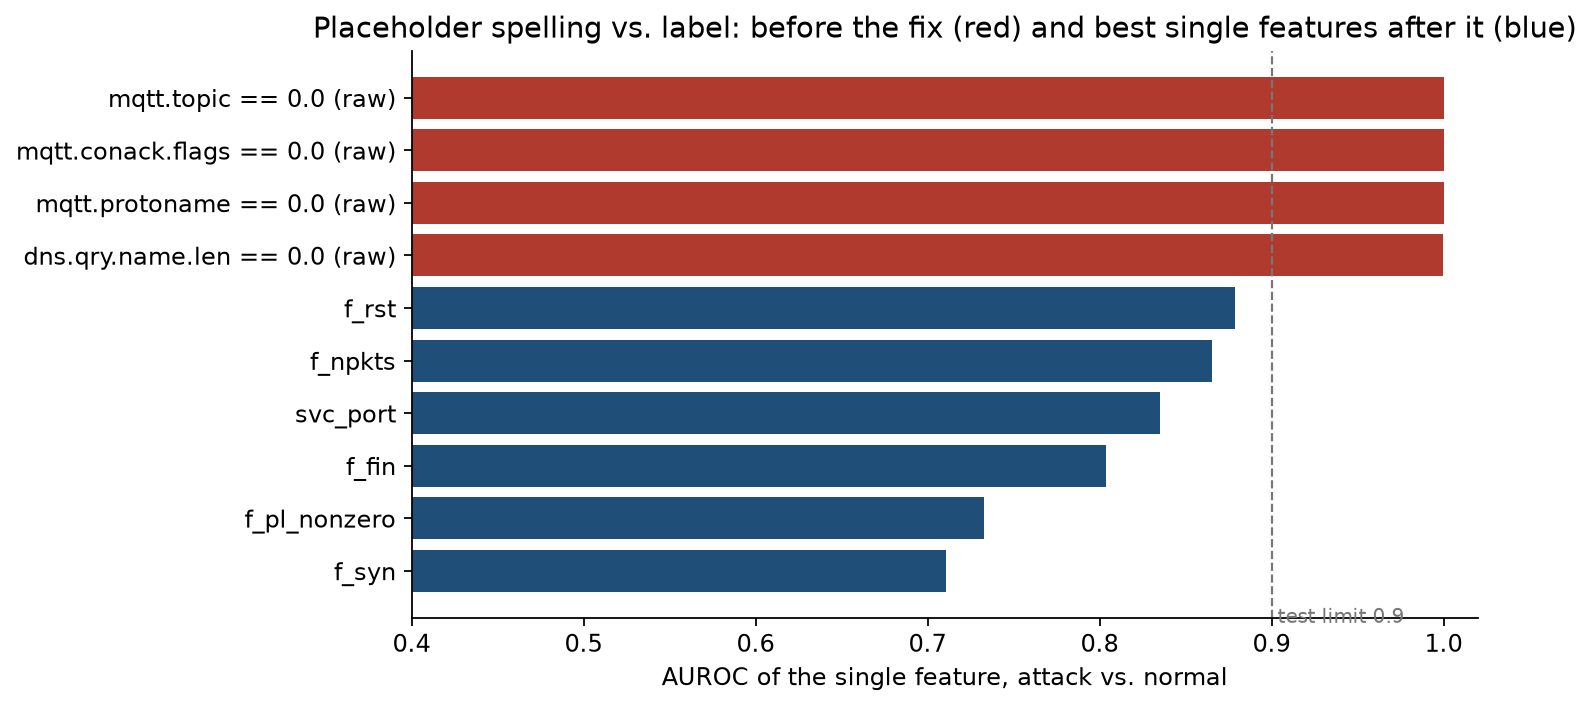
\includegraphics[width=0.8\linewidth]{figures/leak_auroc.png}
\caption{Single-feature AUROC before the placeholder fix (red) and best single features after it (blue)}
\label{fig:leakauroc}
\end{figure}
\begin{figure}[H]
\centering
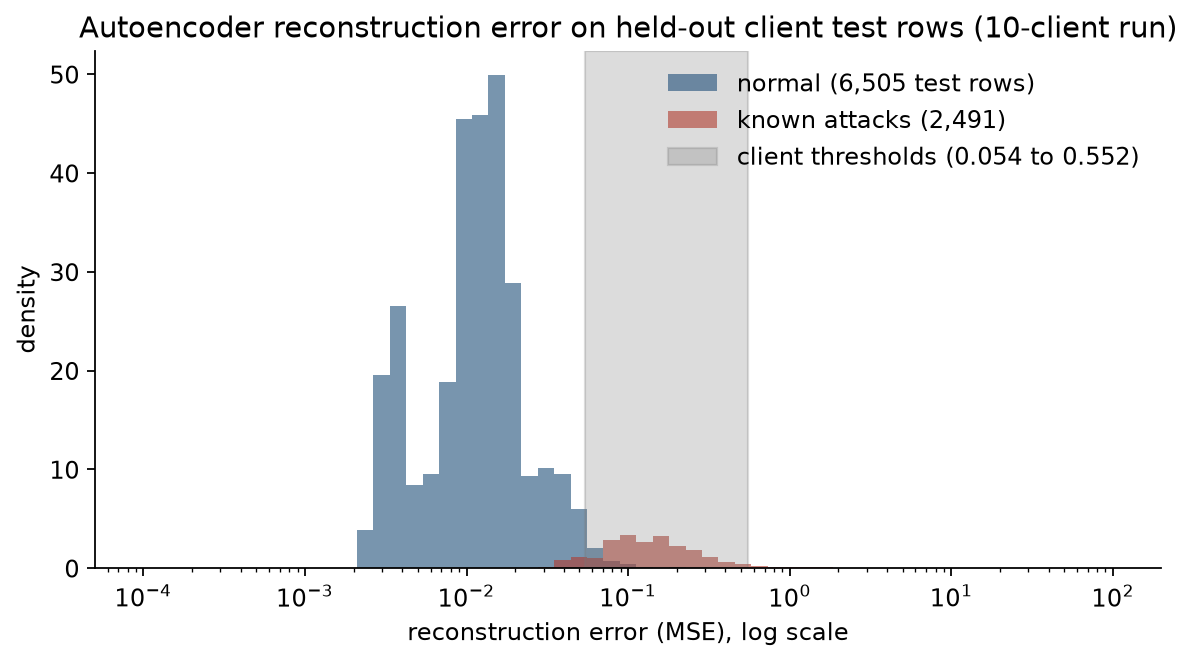
\includegraphics[width=0.8\linewidth]{figures/reconstruction_error.png}
\caption{Autoencoder reconstruction error on held-out client test rows (10-client run); grey band: range of the clients' thresholds}
\label{fig:reconerr}
\end{figure}
\begin{figure}[H]
\centering
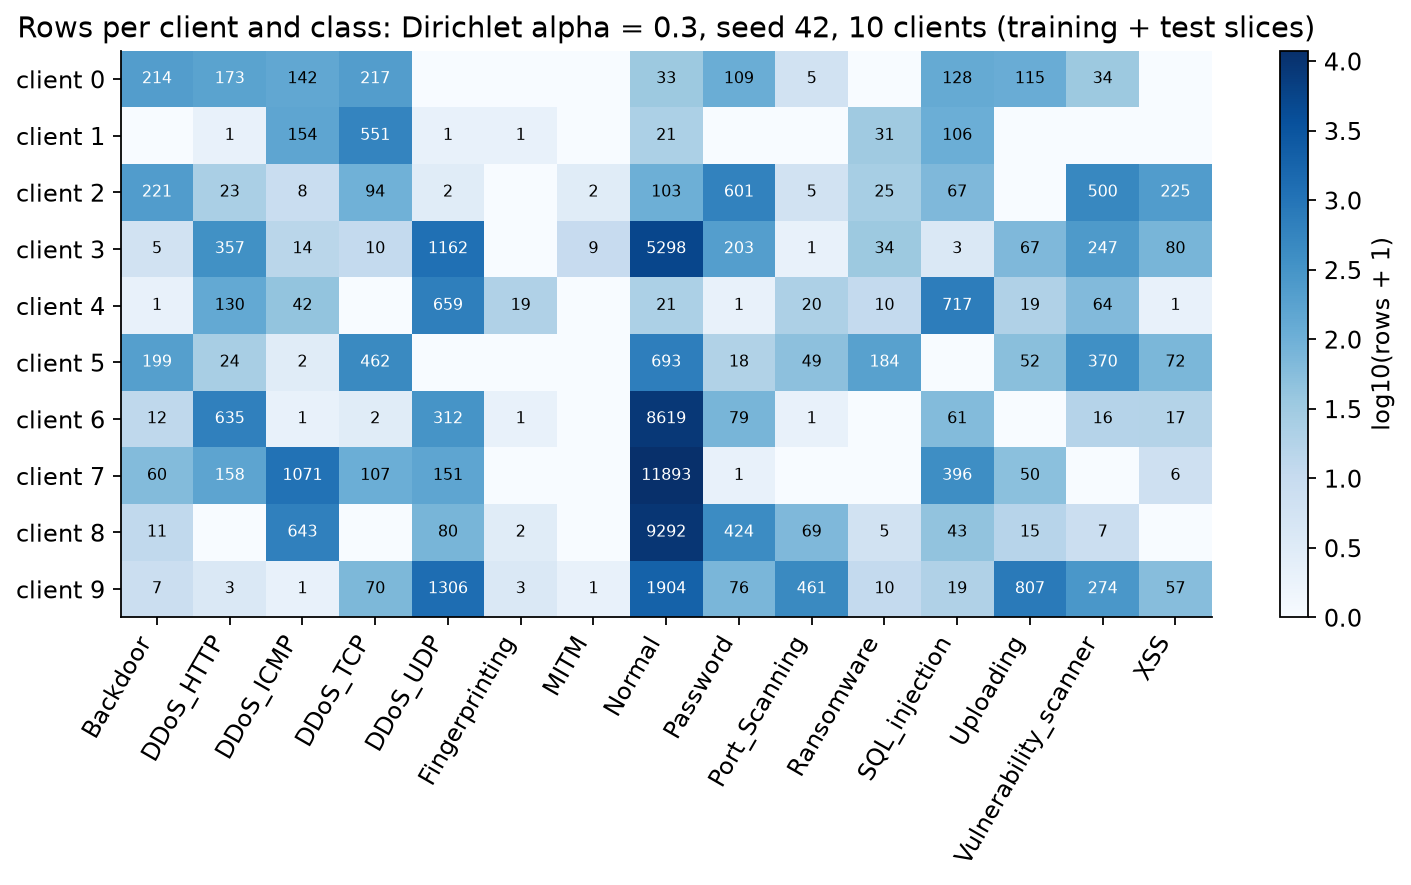
\includegraphics[width=0.98\linewidth]{figures/partition_heatmap.png}
\caption{Rows per client and class for the 10-client run (Dirichlet $\alpha=0.3$, seed 42)}
\label{fig:partheat}
\end{figure}
\begin{figure}[H]
\centering
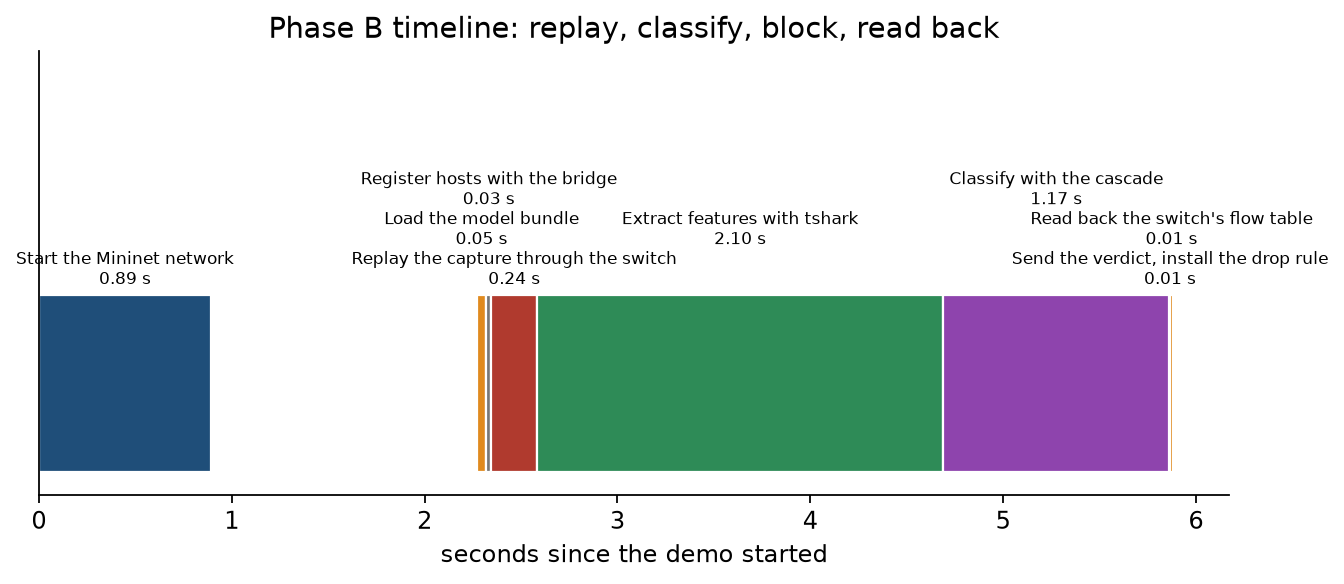
\includegraphics[width=0.9\linewidth]{figures/phase_b_timeline.png}
\caption{Phase B timeline for one replay of the Backdoor capture}
\label{fig:pbtimeline}
\end{figure}

\section{Boosting vs.\ a deep-learning classifier}
On the same 500{,}000-row sample, LightGBM (base features) reached 0.887 macro F1 and a dense MLP of comparable effort (8{,}271 parameters, 15 epochs) reached 0.622. The gap was largest on the application-layer attacks (XSS 0.761 vs.\ 0.072 recall; SQL\_injection 0.767 vs.\ 0.183). This supports the boosting-first design. It is a comparison against a modest baseline, not a claim that deep learning cannot work here.
